\chapter{Keresőfüggvények használata}
\thispagestyle{empty}

A munkalapfüggvények kategóriában találjuk azokat a gyakran
használt függvényeket, amelyek segítségével adatokat
kereshetünk a táblázatban. 

\section{Az FKERES, VKERES függvények}

Az FKERES függvény egy tartomány bal szélső oszlopában
megkeres egy értéket. Ennek az értéknek a sora, és a harmadik
paraméterben megadott tartományon belüli oszlop sorszámának
metszéspontján található cella tartalmát adja eredményül.

Szintaxisa: =FKERES(keresési feltétel;tömb;index;rendezett)

Attól függően, hogy a negyedik, rendezett nevű, opcionális
paraméternek milyen értéket adunk, a függvény eltérően
viselkedik. Amikor az oszlop, amiben keresünk egy értéket nem
rendezett, akkor ennek a paraméternek HAMIS értéket kell adjunk.
Ilyenkor csak pontos egyezés esetén ad eredményt a függvény.
Rendezett oszlop esetén a negyedik paraméter lehet IGAZ, vagy el is
hagyhatjuk. A függvény ilyenkor közelítő eredményt is
adhat. 

Két feladaton keresztül vizsgáljuk meg az FKERES függvény
működését.


\section{20. feladat}

{\itshape
\Aref{20-feladat} ábrán látható táblázat egy üzlet
raktárkészletét mutatja. Minden árut egy kóddal
azonosítanak. Oldjuk meg, hogy egy kódot az A19 cellába írva a
B19:E19 tartományban megjelenjenek az adott áru adatai.}

\begin{figure}[!h]
\begin{center}
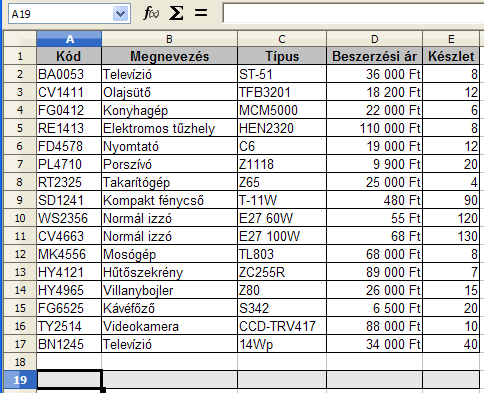
\includegraphics[width=11.804cm]{oocalcv2-img94.png}
\caption{20. feladat}\label{20-feladat}
\end{center}
\end{figure}

A táblázatban létezik egy olyan tartomány, amelynek első
oszlopában kell megkeresni a beírt kód értékét, és
tőle jobbra a második, harmadik, negyedik és ötödik
oszlopból kell megjeleníteni a hozzá tartozó értékeket. Ez
a tartomány az A2:E17.

Írjunk be egy kódot az A19 cellába. A B19 cellában kell, hogy
megjelenjen az e kódhoz tartozó megnevezés. Ebben a cellában
válasszuk a függvénytündért, és az FKERES függvényt
(\ref{20-feladatVLOOKUP} ábra).

\begin{figure}[!h]
\begin{center}
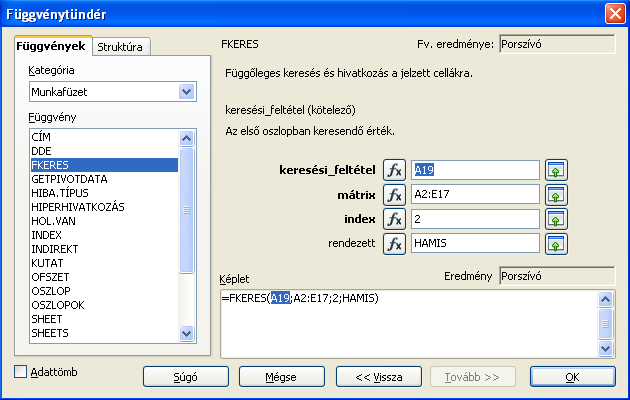
\includegraphics[width=15.999cm]{oocalcv2-img95.png}
\caption{20. feladat -- FKERES függvény}\label{20-feladatVLOOKUP}
\end{center}
\end{figure}

Az első paraméter a keresési feltétel: mit keresünk a tömb
első oszlopában. Esetünkben ez az A19 cella. A második
paraméter maga a tömb. A harmadik, hogy melyik oszlopból kell az
értéket venni. A feladat jellegéből következik, hogy most
pontos egyezésre van szükség, a negyedik paramétert is meg kell
adni: HAMIS. A függvény tehát:
\textsf{\textbf{=FKERES(A19;A2:E17;2;HAMIS)}} (\ref{20-feladatVLOOKUP}
ábra).

A függvény működését a következőképpen
értelmezhetjük: keresd az A19 cella tartalmát az A2:E17
tartomány első oszlopában. Pontos egyezés esetén
jelenítsd meg a megtalált sor és a második oszlop
metszéspontján található cella tartalmát.

A további három cella csak abban különbözik a B19-től,
hogy ott a harmadik, negyedik és ötödik oszlop adatát kell
megjeleníteni. A harmadik, index paramétert kell háromra,
négyre és ötre módosítani. Másolással ez nem oldható
meg. Módosítsuk a hivatkozásokat és másoljuk a cellákat
jobbra. A C19, D19 és az E19 cellákban írjuk át az index
paramétert. A D19 formátumát változtassuk pénznemre, a
tizedesjegyek száma nulla legyen.

\Aref{20-feladatEredmény} ábrán a feladat megoldását látjuk.

\begin{figure}[!h]
\begin{center}
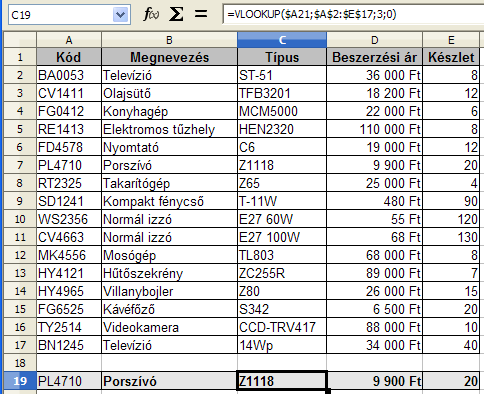
\includegraphics[width=10.104cm]{oocalcv2-img96.png}
\caption{20. feladat -- eredmény}\label{20-feladatEredmény}
\end{center}
\end{figure}

Ellenőrizzük a függvény működését
különböző kódokat írva az A19 cellába. Nem létező
kódot írva a \#HIÁNYZIK hibaüzenetet kapjuk.


\section{21. feladat}

\begin{figure}[!h]
\begin{center}
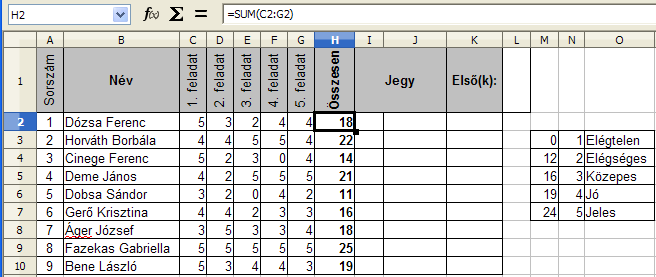
\includegraphics[width=13.999cm]{oocalcv2-img97.png}
\caption{21. feladat}\label{21-feladat}
\end{center}
\end{figure}

{\itshape
\Aref{21-feladat} ábrán egy dolgozat eredményeit látjuk. Az elért
pontszámok alapján függvény segítségével határozzuk meg
minden tanuló osztályzatát. A kritériumokat az M3:O7
cellatartomány tartalmazza: 12 pontig -- Elégtelen (1), 12-től
16 pontig -- Elégséges (2), 16-tól 19-ig -- Közepes (3),
 19-től 24-ig -- Jó (4) és 24 ponttól Jeles (5). A K oszlopban a
legtöbb pontszámot elért tanulók sorában jelenjen meg az
,,Igen'' szó. Az L1 cella azt mutassa,
hogy hány tanuló érte el a legtöbb pontszámot.}

Ennek a feladatnak a megoldásához is az FKERES függvényt fogjuk
használni. Az M3:O7 tartomány első oszlopában fogja
megkeresni a függvény minden tanuló pontszámát. A második,
majd a harmadik oszlopból veszi az osztályzatot. Az M3:O7
tartomány első oszlopa növekvő számsort tartalmaz. Az
FKERES függvény ebben az esetben akkor is ad eredményt, ha nem
talál pontos egyezést, feltéve, hogy az érték a rendezett
lista legalacsonyabb értékénél nagyobb.

Az első tanuló pontszáma 18 pont. Ez a 16 pontnál (Közepes)
több, de a 19 pontnál (Jó) kevesebb, tehát rá a harmadik sor
vonatkozik (\ref{21-feladatVLOOKUP} ábra).

\begin{figure}[!h]
\begin{center}
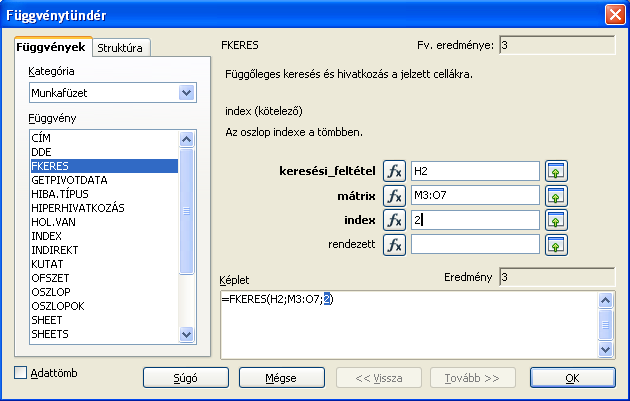
\includegraphics[width=13.999cm]{oocalcv2-img98.png}
\caption{21. feladat --  FKERES függvény}\label{21-feladatVLOOKUP}
\end{center}
\end{figure}

Ebben az esetben a negyedik paramétert nem kell megadni, az
alapértelmezett értéke IGAZ.

A függvény másolása előtt abszolúttá kell tenni a
\textbf{mátrix} paramétert. A végleges képlet tehát:
\textsf{\textbf{=FKERES(H2;\$M\$3:\$O\$7;2)}}.

A J oszlopban a képlet csak a harmadik paraméterben
különbözik. Itt a harmadik oszlopból kell az eredményt venni
(\ref{21-feladatVLOOKUPKéplet} ábra).

\begin{figure}[!h]
\begin{center}
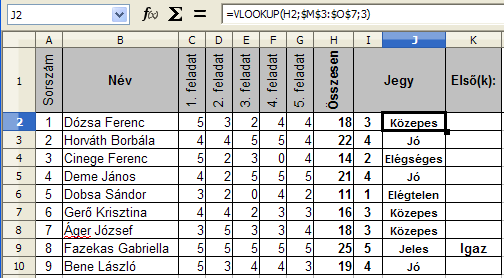
\includegraphics[width=13.333cm]{oocalcv2-img99.png}
\caption{21. feladat --  FKERES függvény képlet}\label{21-feladatVLOOKUPKéplet}
\end{center}
\end{figure}

Ahhoz, hogy a K oszlopban a legtöbb pontszámot elért tanulók
sorában jelenjen meg az ,,Igen''
szó, használhatjuk a HA és a MAX függvényt. A
függvénytündérrel hozzuk létre a következő
kifejezést:
\textsf{\textbf{=HA(MAX(H\$2:H\$10)=H2;"Igen";"")}}.

A legtöbb pontszámot szerzett tanulók számát
kiszámíthatjuk az L1 cellában, összeszámolva az
,,Igen''-ek darabszámát a K oszlopban:
\textsf{\textbf{=DARABTELI(K2:K10;"Igen")}}.

A megoldott feladatot \aref{21-feladatIF} ábrán látjuk.

\begin{figure}[!h]
\begin{center}
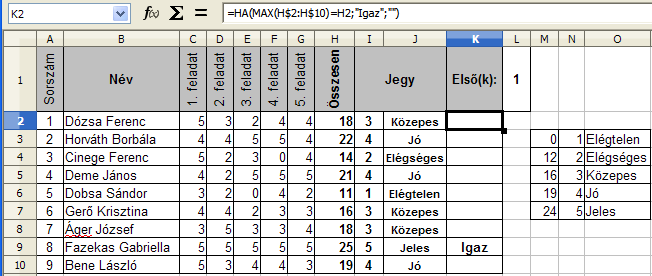
\includegraphics[width=15.999cm]{oocalcv2-img100.png}
\caption{21.  feladat --  HA képlet}\label{21-feladatIF}
\end{center}
\end{figure}

A VKERES függvény pontosan úgy működik, mint az FKERES,
csak a tartomány első oszlopa helyett az első sorban keres.
Erre utal a függvények nevében az első betű: F --
függőleges, V --  vízszintes.


\section{A HOL.VAN és az INDEX függvények}

A \textbf{HOL.VAN} függvény a keresett elem tömbben elfoglalt
pozícióját adja vissza. A tömb egy sorból vagy egy
oszlopból állhat. Szintaxisa: HOL.VAN(keresési
feltétel;keresési\_tartomány;típus). A harmadik
\textbf{típus} paraméternek 0 értéket kell adni, ha pontos
egyezést keresünk. Amikor több ilyen is van, az első
találatot adja eredményül. -1 esetén a függvény
feltételezi, hogy a tömb csökkenő rendbe rendezett. Ilyenkor
az első nagyobb vagy egyenlő értéket adja vissza.

A harmadik paraméter elhagyása, vagy 1 értéke esetén a
függvény az utolsóként előforduló, a keresési
feltételnél kisebb vagy azzal egyenlő értéket adja vissza.

Egy egyszerű példán könnyen megérthetjük a függvény
működését. Az előző feladat táblázatában
 találjuk meg, hogy a névsorban hányadik diák érte el a
legkevesebb pontszámot.

\Aref{MATCHFüggvény} ábrán látjuk, hogy az első paraméter a MIN(H2:H10)
függvény, ami megadja a legkisebb számot a H2:H10 tartományban.
Ennek a számnak a sorszámát találja meg a HOL.VAN függvény,
mert keresési tartomány is a H2:H10. Látjuk, hogy az eredmény
5, tehát a névsorban az ötödik  tanuló érte el a
legkevesebb pontszámot.

\begin{figure}[!h]
\begin{center}
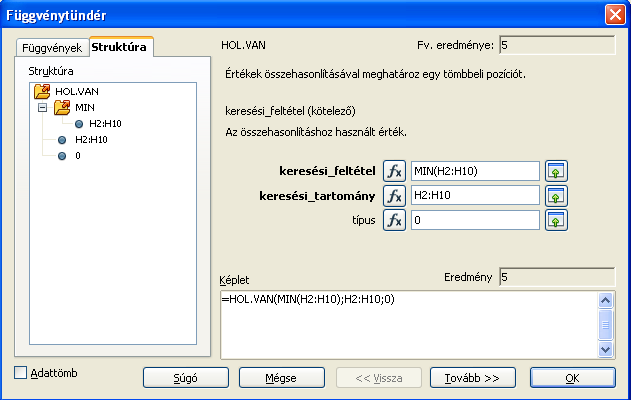
\includegraphics[width=15.999cm]{oocalcv2-img101.png}
\caption{HOL.VAN függvény struktúrája}\label{MATCHFüggvény}
\end{center}
\end{figure}

Az \textbf{INDEX} függvény adott sor és oszlop
találkozásánál lévő cella tartalmát adja
eredményül. Szintaxisa: INDEX(hivatkozás;sor;oszlop;tartomány).
Amennyiben a hivatkozás több tartományból  áll,
zárójelek között kell megadni. A negyedik paraméter
opcionális, csak akkor kell megadni, ha  több tartományból
áll a hivatkozás.

A HOL.VAN függvényt gyakran használják az INDEX beágyazott
függvényeként. Olyan keresési feladatokat is megoldhatunk
ezekkel a függvényekkel, amelyeket az FKERES, VKERES
függvényekkel nem. A következő feladatban vizsgáljunk meg
egy ilyen esetet.


\section{22. feladat}

{\itshape
\Aref{22-feladat} ábrán az A oszlopban dátumértékek, a C oszlopban az
adott napi bevétel van feltüntetve. A C15 cellában jelenítsük
meg legnagyobb bevételt, a C20-ban pedig hozzá tartozó
dátumot.}

\begin{figure}[!h]
\begin{center}
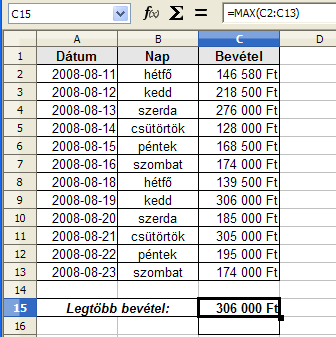
\includegraphics[width=8.888cm]{oocalcv2-img102.png}
\caption{22. feladat}\label{22-feladat}
\end{center}
\end{figure}

A táblázatot megfigyelve láthatjuk, hogy itt a C oszlopban kell
megkeresni egy értéket és a tőle balra lévő oszlopból
megjeleníteni a hozzá tartozó tartalmat. Az FKERES függvényt
ezért itt nem használhatjuk, illetve csak akkor, ha segédoszlopot
alkalmazunk, másolatot készítve az A2:A13 tartományról a
bevétel oszlopától jobbra, például a D oszlopba. Amikor nem
alkalmazhatjuk ezt a módszert, más függvényt kell
használnunk.

A HOL.VAN függvénnyel keressük meg melyik sorban van a legnagyobb
szám a B2:B12 tartományban, és ez lesz az INDEX függvény sor
paramétere. Az oszlop paraméter 1 lesz, a tartomány pedig az
A2:C13.

A függvénytündér segítségével hozzuk létre a
kifejezést (\ref{INDEXFüggvény} ábra).

\begin{figure}[!h]
\begin{center}
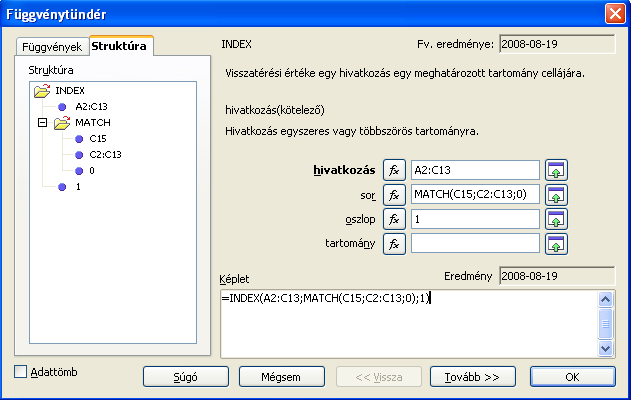
\includegraphics[width=15.999cm]{oocalcv2-img103.png}
\caption{22. feladat INDEX függvény struktúrája}\label{INDEXFüggvény}
\end{center}
\end{figure}

